% !TEX root = ../main.tex

We tackle Problem \ref{BehaviorSynthesisProblem} in two sequential steps.

\subsection{Reactive LTL Synthesis}

First, we automatically generate a correct-by-construction symbolic automaton from the formal specification $\mathcal{T}_S$ using \textsc{gr(1)} synthesis (Section \ref{S:GR1}, \cite{Bloem2012GR1}).
Specifically, we use the tool $\mathtt{slugs}$ \cite{SLUGS}, which implements a synthesis algorithm introduced by Raman, et al. \cite{Vasu2013ICRA, Vasu2015TRO}.
Their algorithm can handle a fragment of \textsc{ltl} slightly larger than \textsc{gr(1)}.
Namely, the one that includes $\LTLX$ (next) operators in liveness formulas, such as formulas \eqref{ActionFairnessConditionsFormula} and \eqref{TopologyFairnessConditionsFormula} in Section \ref{S:ltl}.
If the formal specification, $\mathcal{T}_S$, is realizable, we can extract a finite-state automaton.
An example is provided in Fig. \ref{Fig:SynthesizedAutomaton}.

\textsc{Gr(1)} synthesis is quadratic in the size of the state space \cite{Bloem2012GR1}, which in turn is exponential in the number of atomic propositions (known as the state explosion problem).
Thus, one concern might be that the introduction of outcome (Section \ref{S:AP}) and memory (Section \ref{S:ltl-goals}) propositions will increase the state space by a factor of $O(2^{k | \mathcal{Y} | + | \mathcal{G} | })$, where $k$ is the number of outcomes corresponding to each capability ($k=2$ if $Out(y) = \{ c, f \}$, $\forall y \in \mathcal{Y}$).
However, while the state space definitely grows in size, the increase is far from worst-case exponential, because the outcome propositions are tied to the corresponding activation propositions via the environment safety assumptions (Section \ref{S:ltl}).
In addition, the activation of actions is also constrained by formula \eqref{PreconditionsFormula}, when they have preconditions.
Likewise, memory propositions are also highly constrained by formulas \eqref{MemoryFormula} or \eqref{GoalOrderFormula}.
For these reasons, an exponential blow-up is mitigated in practice.

\begin{figure}[t]
\centering
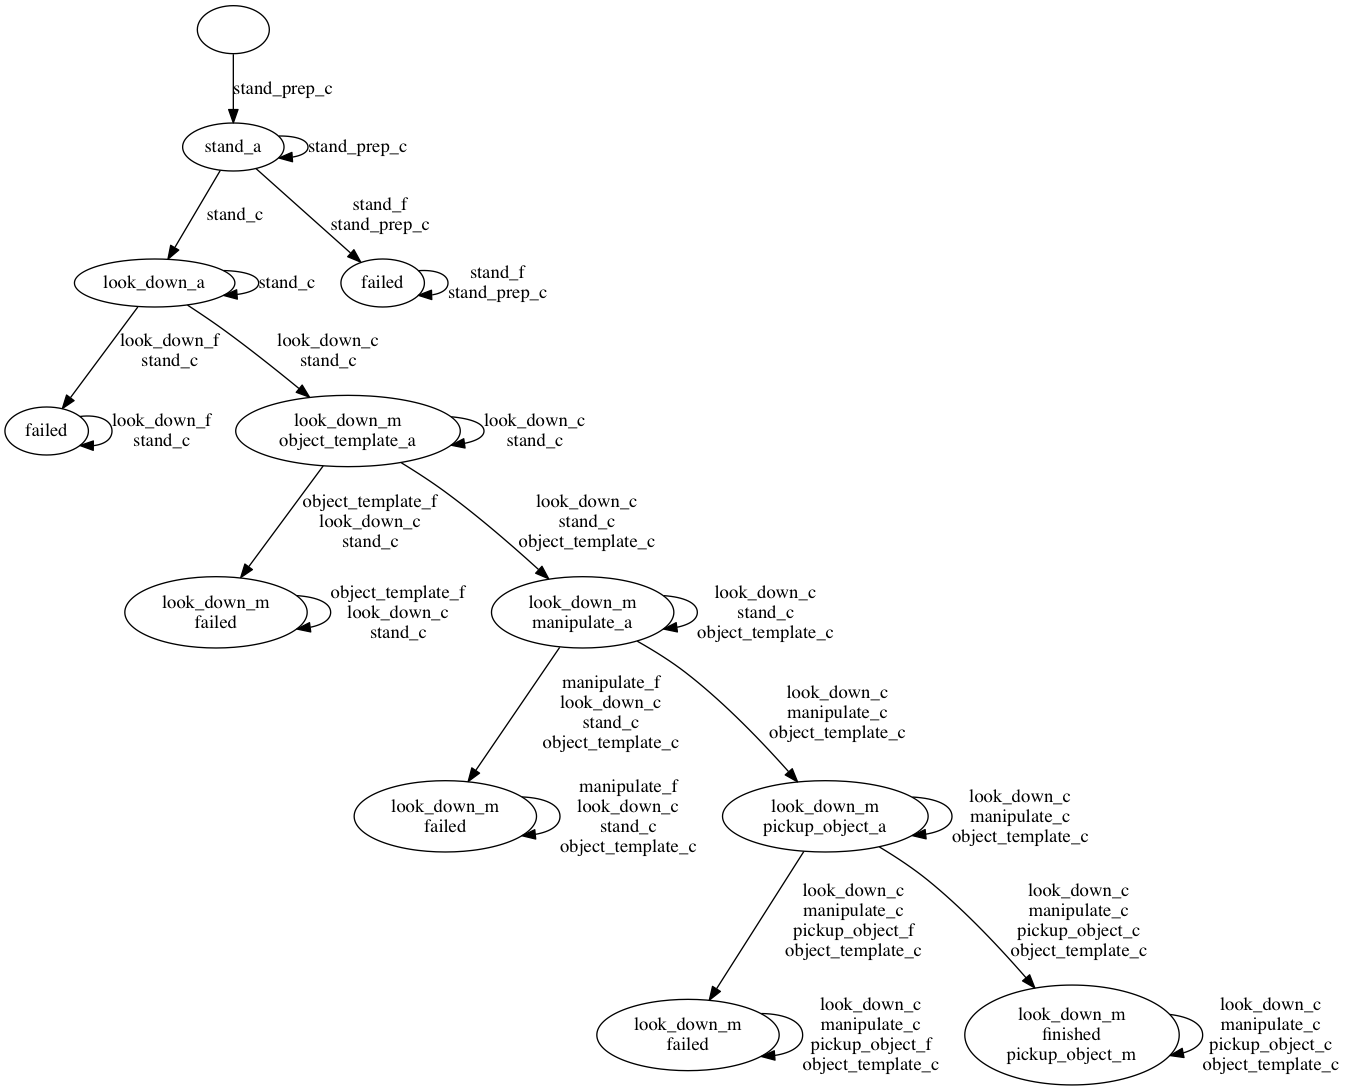
\includegraphics[width=0.95\columnwidth,clip]{./img/synthesized_automaton.png}
\caption{
	The output of \textsc{gr(1)} synthesis is a symbolic finite-state automaton.
	For clarity, only the atomic propositions that are $\True$ are depicted.
	The formal specification was generated from the user input $\mathcal{I} = \{ \mathtt{stand\_prep} \}$ and $\mathcal{G} = \{ \mathtt{look\_down, pickup\_object} \}$, according to Section \ref{S:ltl}.
	We will revisit this example in Section \ref{S:SynthesisFromScratch}.
	In general, the synthesized automata are not tree-like structures.
	This is an artifact of our choice of formulas in Section \ref{S:ltl-goals}.
}
\label{Fig:SynthesizedAutomaton}
\end{figure}

\subsection{Proposition Grounding \& State Machine Instantiation}

Second, we use the mapping $\gamma: \mathcal{D} \rightarrow \mathcal{C}$ to automatically generate code that instantiates the symbolic automaton.
Without loss of generality, we generate executable state machines in the FlexBE framework introduced in Section \ref{S:FlexBE}.
Thus, the primitive system capabilities $\mathcal{C}$ are invoked via the execution of parametrized FlexBE states $Q_P$.

Specifically, activation propositions $\pi_y \in \mathcal{Y}$, $y \in \{ a, m \}$, that evaluate to $\True$ in a state of the synthesized automaton are instantiated as a state $q_p \in Q_P$ in the FlexBE state machine.
Furthermore, the corresponding outcome propositions $\pi_y^o \in \mathcal{X}$, $o \in Out(y)$, are mapped to the outcomes of that state, $Out(q_p)$.
In practice, an outcome proposition can correspond to multiple outcomes of the state implementation.
The auxiliary memory propositions introduced in Section \ref{S:ltl-goals} were only necessary for the specification and synthesis steps.
They do not have to be instantiated in software.
Finally, in the finite run case, the outcome propositions $\pi_{Exec}^o \in \mathcal{Y}$, $o \in Out(Exec)$, are mapped to the outcomes of the FlexBE state machine, $Out(SM)$.
The transitions of the synthesized automaton are mapped to those of the state machine.
%(after some extra processing where, e.g., we group all of the $\mathtt{failed}$ states in Fig. \ref{Fig:SynthesizedAutomaton} together).
Examples of FlexBE state machines generated using our behavior synthesis approach are provided in Section \ref{S:experiments}.

% END